\chapter{Técnicas de laboratorio II: síntesis y análisis en la práctica}\label{ch:b2:lab-techniques-2}

Una reacción de Grignard fracasa un lunes por la mañana: el matraz se había enjuagado pero no secado, y las pocas
gotas de agua que quedaban destruyeron el reactivo a medida que se formaba. Repetida en material secado en estufa,
bajo nitrógeno, añadiendo el haluro gota a gota a un matraz agitado y enfriado, la misma reacción
funciona. La química no cambió; cambió el montaje. Este capítulo trata de la práctica que convierte una
reacción sobre el papel en un producto en un vial: controlar la reacción, mantener fuera el aire y el agua,
aislar el producto bruto, purificarlo y demostrar qué se ha obtenido.

\begin{omfigure}
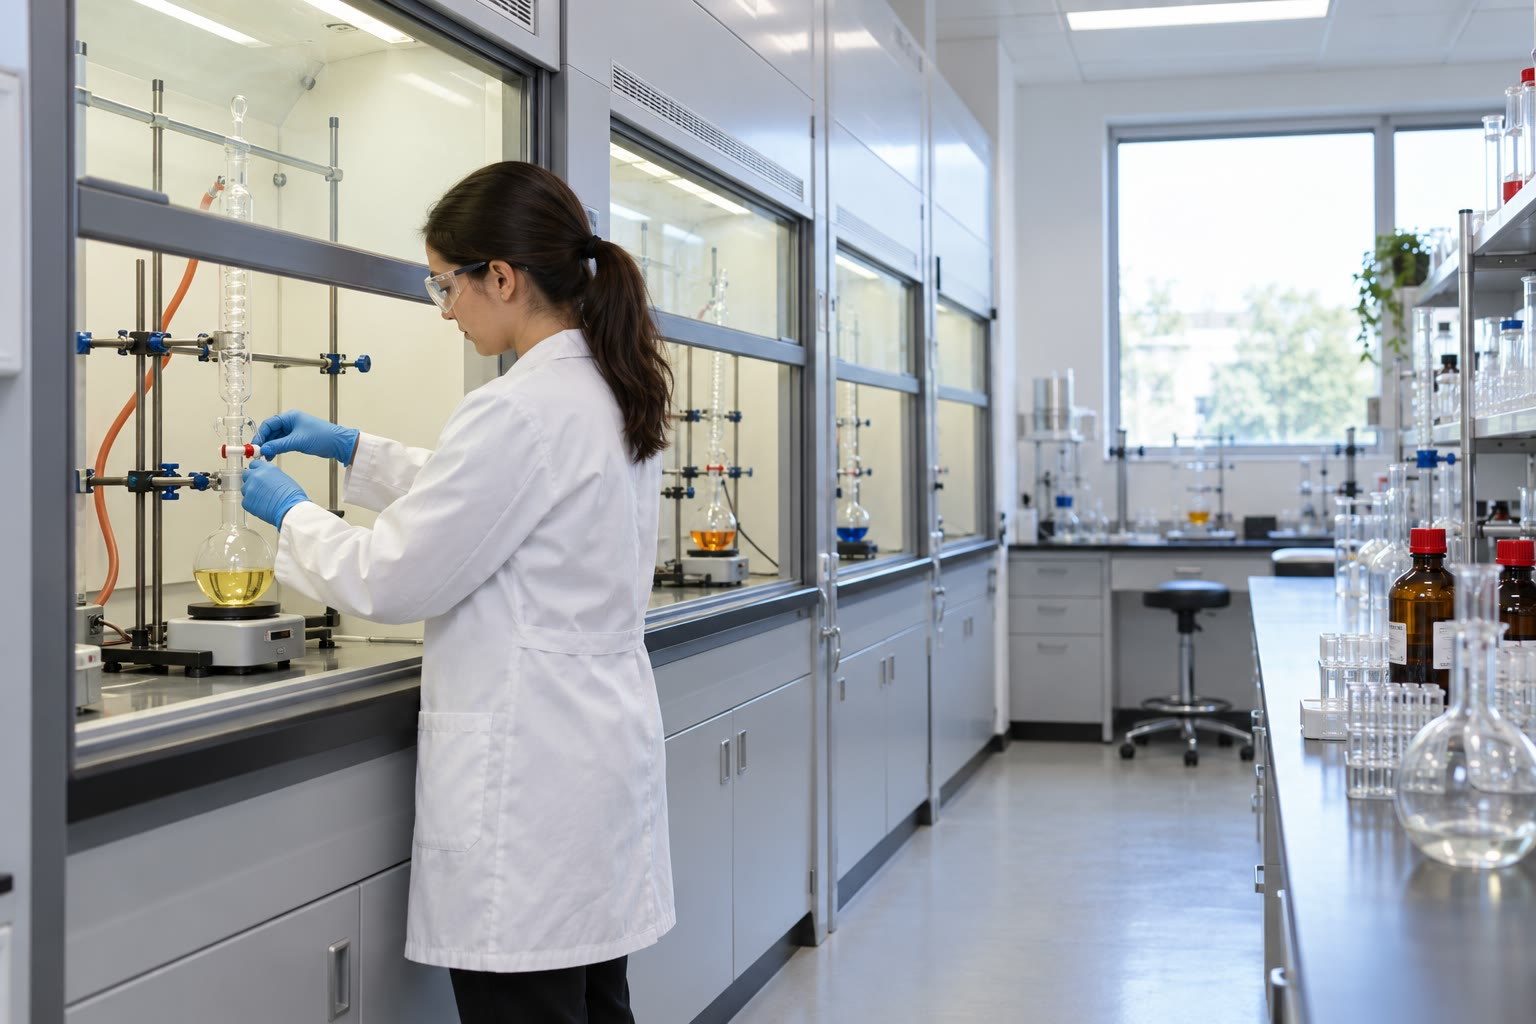
\includegraphics[width=0.56\linewidth]{images/book3/ai/b2-35-synthesis-lab.jpg}

{\small Un laboratorio de síntesis orgánica: reacciones en vitrinas de gases, matraces sujetos con pinzas a soportes
(ilustración).}
\end{omfigure}

\begin{recall}
El volumen del primer año: peligros y pictogramas SGA, extracción, recristalización, destilación, \omterm{def:b2:chromatography:principle}{cromatografía} en capa
fina y $R_f$, punto de fusión, reactivos de Grignard. \Cref{ch:b2:reaction-enthalpy}: \omterm{def:b2:reaction-enthalpy:reaction-quantity}{entalpía de
reacción} y \omterm{def:b2:continuous-reactors:adiabatic-rise}{aumento adiabático de temperatura}. \Cref{ch:b2:chromatography},
\cref{ch:b2:structure-determination} y \cref{ch:b2:measurement-statistics}: el análisis.
\end{recall}

\section{Llevar a cabo una reacción bajo control}

Una reacción en un matraz libera su calor allí donde se produce. El químico controla la temperatura con un baño
(hielo y agua, hielo y sal, hielo seco y acetona para las temperaturas más bajas), con el reflujo de un
disolvente en ebullición, que limita la temperatura a su punto de ebullición mientras el refrigerante devuelve el
vapor, y con la velocidad a la que se añade un reactivo. Un termómetro interno, en el líquido y no
en el baño, mide lo que importa.

\begin{proposition}[Acumulación]\label{prop:b2:lab-techniques-2:accumulation}
Si un reactivo se añade más deprisa de lo que reacciona, la cantidad sin reaccionar $n_{\mathrm{acc}}$ se acumula. Si
llegara a reaccionar de golpe, sin refrigeración, la temperatura de la mezcla de capacidad calorífica $C$ aumentaría en
\begin{equation*}
\Delta T_{\mathrm{ad}} = \frac{n_{\mathrm{acc}}\,|\Delta_rH|}{C}.
\end{equation*}
\end{proposition}

\begin{proof}
La reacción de $n_{\mathrm{acc}}$ libera $n_{\mathrm{acc}}|\Delta_rH|$ a presión constante
(\cref{ch:b2:reaction-enthalpy}); sin intercambio de calor, todo él calienta la mezcla, como en la
\omterm{def:b2:reaction-enthalpy:flame-temperature}{temperatura adiabática de llama} (\cref{def:b2:reaction-enthalpy:flame-temperature}): $C\Delta T =
n_{\mathrm{acc}}|\Delta_rH|$.
\end{proof}

El peligro es máximo cuando una reacción tarda en arrancar, como ocurre a menudo con la formación de los reactivos de Grignard: el haluro
añadido antes de la iniciación se acumula y, cuando la reacción arranca por fin, se embala. La regla es añadir una pequeña
porción, ver cómo arranca la reacción (calentamiento, turbidez, reflujo suave) y solo entonces añadir el resto al
ritmo que la refrigeración pueda seguir.

\section{Condiciones anhidras y atmósfera inerte}

\begin{definition}[Atmósfera inerte]\label{def:b2:lab-techniques-2:inert}
Una reacción se lleva a cabo en \emph{atmósfera inerte}\index{atmosfera inerte@atmósfera inerte} cuando el aire del aparato
se ha sustituido por un gas poco reactivo, nitrógeno o argón, mantenido a una ligera sobrepresión para que el aire
no pueda entrar.
\end{definition}

Los reactivos organometálicos, los hidruros metálicos y muchos catalizadores reaccionan con el agua y el oxígeno. El material de vidrio se
seca en estufa y se monta caliente, o se flamea bajo una corriente de gas; los disolventes se compran anhidros o se secan
sobre un reactivo que reacciona con el agua; los líquidos se transfieren con jeringas a través de septos de goma.
El gas sale por un borboteador de aceite, que muestra el caudal e impide el retroceso del aire. La
rampa de Schlenk y la caja de guantes, para los compuestos más sensibles, se verán en el volumen del tercer año.

\begin{omfigure}
\begin{tikzpicture}[lab/.style={font=\scriptsize, align=center}]
\fill[omDef!10] (-1.7,-0.3) rectangle (1.7,1.0);
\draw[om glass] (-1.7,1.2) -- (-1.7,-0.3) -- (1.7,-0.3) -- (1.7,1.2);
\foreach \x/\y in {-1.5/0.0,-1.45/0.55,1.3/0.05,1.3/0.6,-1.25/0.3,1.05/-0.15}{
  \draw[omDef!50, fill=white] (\x,\y) rectangle ++(0.18,0.18);}
\pic (f) at (0,0) {threeneck={0.35}{omThm!25}};
\pic[rotate=25] (d) at (f-l) {dropfunnel={0.5}{omMeth!20}};
\pic (c) at (f-c) {condenser};
\pic[rotate=-25] (t) at (0.0,0.42) {thermometer};
\pic (b) at (3.6,3.6) {bubbler};
\draw[thick, black!60] (0,6.25) -- (0,6.75) -- (3.25,6.75) -- (b-in);
\coordinate (dtop) at ($(f-l)+(-1.52,3.26)$);
\draw[thick, black!60] (dtop) -- ++(0,0.35) -- ++(-0.9,0) node[left, lab] {N$_2$};
\node[lab, anchor=north] at (0,-0.4) {baño de hielo};
\node[lab, anchor=east] at (-1.9,2.6) {embudo de\\adición};
\node[lab, anchor=west] at (0.55,5.0) {refrigerante};
\node[lab, anchor=west] at (1.75,2.6) {termómetro\\(interno)};
\node[lab, anchor=north] at (3.6,3.45) {borboteador (salida de gas)};
\end{tikzpicture}
\par\vspace{4pt}

{\small Una reacción bajo nitrógeno (esquema). Matraz de tres bocas en un baño de hielo, con un termómetro
interno en el líquido; el reactivo se añade desde un embudo de presión compensada por el que entra el
nitrógeno; el gas sale por el refrigerante y un borboteador de aceite.}
\end{omfigure}

\begin{method}[Montar una reacción anhidra bajo nitrógeno]\label{met:b2:lab-techniques-2:anhydrous}
\begin{enumerate}
  \item Séquese el material de vidrio en estufa y móntese en caliente, engrasando o enfundando las juntas; colóquense un septo
        o el embudo de adición, el refrigerante y el borboteador.
  \item Púrguese con nitrógeno mientras se enfría; manténgase un flujo lento (una burbuja cada uno o dos segundos) durante todo el proceso.
  \item Añádanse los sólidos antes de purgar, y los disolventes anhidros y los reactivos líquidos con jeringa o cánula a través de un
        septo.
  \item Enfríese o caliéntese según lo previsto; empiécese la adición con una pequeña porción y compruébese que la reacción
        arranca antes de continuar.
\end{enumerate}
\end{method}

\section{Tratamiento final}

\begin{definition}[Tratamiento final]\label{def:b2:lab-techniques-2:work-up}
El \emph{tratamiento final}\index{tratamiento final} de una reacción es la secuencia de operaciones, posterior a la reacción, que
convierte la mezcla de reacción en el producto bruto: extinción, extracción y lavado, secado,
filtración y evaporación del disolvente.
\end{definition}

\begin{definition}[Extracción ácido--base]\label{def:b2:lab-techniques-2:acid-base-extraction}
Una \emph{extracción ácido--base}\index{extraccion acido--base@extracción ácido--base} separa compuestos orgánicos ácidos, básicos y neutros
disueltos en un disolvente orgánico lavando la disolución con ácidos o bases acuosos, que
convierten una clase de compuestos en iones que pasan al agua.
\end{definition}

\begin{proposition}[Quién va adónde]\label{prop:b2:lab-techniques-2:acid-base-extraction}
El hidrogenocarbonato de sodio acuoso (pH 8.3) extrae un ácido carboxílico ($\mathrm pK_a$ de unos 4) pero no un
fenol ($\mathrm pK_a$ de unos 10), que necesita hidróxido de sodio; el ácido clorhídrico diluido extrae una
amina cuyo ácido conjugado tiene un $\mathrm pK_a$ de 4.6 o más; los compuestos neutros permanecen en la capa
orgánica.
% ledger: ph:NaHCO3, pka:benzoic, pka:phenol, pka:anilinium
\end{proposition}

\begin{proof}
Una especie está principalmente en su forma básica cuando $\mathrm{pH} > \mathrm pK_a$, y en más del 99~\% cuando
$\mathrm{pH} > \mathrm pK_a + 2$. A pH 8.3, el ácido benzoico (4.2) está en más del 99~\% como benzoato, un ion
que permanece en el agua; el fenol (9.99) está en alrededor del 2~\% como fenóxido ($10^{8.3 - 10.0}$) y permanece esencialmente
en la capa orgánica, hacia la que se reparte la forma neutra. En hidróxido de sodio (pH superior a 12) el fenol se
convierte en fenóxido. En ácido clorhídrico diluido (pH de alrededor de 1), la anilina (anilinio 4.6) está en más del
99~\% como anilinio. Cada ion, una vez en el agua, se recupera llevando el pH en el otro sentido, lo que
regenera el compuesto neutro, y extrayéndolo de nuevo.
\end{proof}

\begin{omfigure}
\begin{tikzpicture}[x=1cm, y=1cm, st/.style={draw=black!70, rounded corners=2pt, fill=white,
  font=\scriptsize, align=center, inner sep=3pt, text width=3.0cm}, ar/.style={->, thick, black!70}]
\node[st, fill=omDef!10] (m) at (0,0) {ácido benzoico, fenol,\\anilina, naftaleno\\en etoxietano};
\node[st, fill=omThm!10] (a1) at (5.0,0) {acuosa: benzoato\\$\to$ HCl $\to$ ácido benzoico};
\node[st] (o1) at (0,-1.6) {fenol, anilina,\\naftaleno};
\node[st, fill=omThm!10] (a2) at (5.0,-1.6) {acuosa: fenóxido\\$\to$ HCl $\to$ fenol};
\node[st] (o2) at (0,-3.2) {anilina, naftaleno};
\node[st, fill=omThm!10] (a3) at (5.0,-3.2) {acuosa: anilinio\\$\to$ NaOH $\to$ anilina};
\node[st, fill=omMeth!10] (o3) at (0,-4.8) {naftaleno\\(secar, evaporar)};
\draw[ar] (m) -- node[above, font=\tiny] {con NaHCO$_3$} (a1);
\draw[ar] (m) -- (o1); \draw[ar] (o1) -- node[above, font=\tiny] {con NaOH} (a2);
\draw[ar] (o1) -- (o2); \draw[ar] (o2) -- node[above, font=\tiny] {con HCl} (a3);
\draw[ar] (o2) -- (o3);
\pic at (8.6,-3.6) {sepfunnel={omDef!25}{omThm!20}};
\node[font=\scriptsize, align=center] at (8.6,-4.0) {embudo de decantación};
\end{tikzpicture}
\par\vspace{4pt}

{\small Separación ácido--base de cuatro compuestos (\cref{prop:b2:lab-techniques-2:acid-base-extraction}).
La capa orgánica (columna izquierda) pierde una clase en cada lavado; cada extracto acuoso (derecha) devuelve
su compuesto cuando se invierte el pH.}
\end{omfigure}

\begin{definition}[Agente desecante]\label{def:b2:lab-techniques-2:drying-agent}
Un \emph{agente desecante}\index{agente desecante} es una sal anhidra, como el sulfato de magnesio o de sodio,
que fija como agua de hidratación el agua disuelta en una disolución orgánica y que después se elimina por
filtración.
\end{definition}

\begin{method}[Del matraz de reacción al producto bruto]\label{met:b2:lab-techniques-2:work-up}
\begin{enumerate}
  \item Extíngase: destrúyanse los reactivos aún activos con una disolución acuosa adecuada, lentamente y
        enfriando.
  \item Extráigase con un disolvente orgánico; sepárense las capas (compruébese cuál es cuál añadiendo una gota de
        agua); vuélvase a extraer la capa acuosa.
  \item Lávense las capas orgánicas reunidas (ácido, base y luego salmuera, una disolución saturada de cloruro de sodio
        que elimina la mayor parte del agua disuelta).
  \item Séquese con un \omterm{def:b2:lab-techniques-2:drying-agent}{agente desecante} hasta que una parte de él quede suelta; fíltrese.
  \item Elimínese el disolvente en un evaporador rotatorio a presión reducida; pésese el producto bruto.
\end{enumerate}
\end{method}

\section{Purificación}

\begin{definition}[Cromatografía flash]\label{def:b2:lab-techniques-2:flash}
La \emph{cromatografía flash}\index{cromatografia flash@cromatografía flash} es una \omterm{def:b2:chromatography:principle}{cromatografía} preparativa en columna sobre sílice en
la que el eluyente se impulsa a través de la columna mediante una ligera presión de gas, de modo que una separación de gramos
de material dura minutos; el eluyente se elige por \omterm{def:b2:chromatography:principle}{cromatografía} en capa fina sobre la misma sílice.
\end{definition}

\begin{proposition}[Volúmenes de columna]\label{prop:b2:lab-techniques-2:column-volumes}
Un compuesto que corre con un $R_f$ dado en una placa de CCF sale de una columna de la misma sílice y el mismo eluyente tras
aproximadamente $1/R_f$ volúmenes de columna de eluyente.
\end{proposition}

\begin{proof}[Argumento]
En la placa el compuesto recorre $R_f$ veces la distancia del frente del disolvente: su velocidad media es $R_f$
veces la del eluyente. En la columna el mismo reparto da la misma razón de velocidades, de modo que el
compuesto necesita $1/R_f$ veces el volumen de eluyente que llena la columna (el volumen muerto) para
salir; en el lenguaje del \cref{ch:b2:chromatography}, $R_f \approx 1/(1 + k)$. Un compuesto con $R_f = 0.25$
sale tras unos cuatro volúmenes de columna, bien separado de uno con 0.5 (dos volúmenes).
\end{proof}

\begin{omfigure}
\begin{tikzpicture}[lab/.style={font=\scriptsize, align=left, anchor=west}]
\pic (k) at (0,0) {chromcolumn={3.4}};
\node[lab] at (0.6,4.6) {eluyente};
\node[lab] at (0.6,3.55) {arena};
\node[lab] at (0.6,2.2) {lecho de sílice};
\foreach \i/\c in {0/white, 1/omThm!25, 2/omThm!25, 3/white, 4/omDef!25, 5/omDef!25, 6/white}{
  \pic at ({2.4+0.55*\i},-1.2) {testtube={0.45}{\c}};}
\node[font=\scriptsize] at (4.05,-1.6) {fracciones 1 a 7};
\pic at (7.6,-1.2) {tlcplate};
\foreach \j/\x in {2/7.15,3/7.45,5/7.75,6/8.05}{\node[font=\tiny] at (\x,-1.38) {\j};}
\fill[omThm] (7.45,0.95) circle (0.06); \fill[omThm] (7.15,0.95) circle (0.06);
\fill[omDef] (8.05,-0.05) circle (0.06); \fill[omDef] (7.75,-0.05) circle (0.06);
\node[font=\scriptsize, align=center] at (7.6,2.15) {CCF de las\\fracciones};
\end{tikzpicture}
\par\vspace{4pt}

{\small \omterm{def:b2:lab-techniques-2:flash}{Cromatografía flash} (esquema). El producto bruto se deposita sobre la sílice y se eluye;
el eluido se recoge en fracciones; una placa de CCF de las fracciones muestra dónde ha salido cada compuesto
(aquí, el compuesto rápido y apolar en las fracciones 2--3, y el más lento en las 5--6), y las fracciones puras se
reúnen.}
\end{omfigure}

\begin{method}[Realizar una columna flash]\label{met:b2:lab-techniques-2:flash}
\begin{enumerate}
  \item Elíjase el eluyente por CCF: el compuesto deseado con un $R_f$ de 0.25--0.35, aproximadamente, lo más lejos posible de
        las impurezas.
  \item Rellénese la columna con sílice (de 30 a 100 veces la masa de producto bruto, aproximadamente) en suspensión o en seco; añádase una capa
        de arena.
  \item Deposítese el producto bruto en el mínimo volumen de disolvente (o adsorbido sobre un poco de sílice).
  \item Elúyase a ligera presión; recójanse fracciones; compruébense por CCF; reúnanse las puras y
        evapórense.
\end{enumerate}
\end{method}

Los líquidos que se descomponen cerca de su punto de ebullición se destilan a presión reducida, donde hierven
a menor temperatura.

\begin{definition}[Destilación a presión reducida]\label{def:b2:lab-techniques-2:reduced-pressure}
Una \emph{destilación a presión reducida}\index{destilacion a presion reducida@destilación a presión reducida} se lleva a cabo
en un aparato conectado a una bomba de vacío a través de un manómetro, a una presión a la que el líquido hierve a una
temperatura que puede soportar.
\end{definition}

\begin{proposition}[Ebullición a presión reducida]\label{prop:b2:lab-techniques-2:reduced-pressure}
Con $T_b$ la temperatura de ebullición a la presión de referencia $p^\circ$ y $\Delta_{\mathrm{vap}}H$
tratada como constante, la temperatura de ebullición a la presión $p$ viene dada por
\begin{equation*}
\frac{1}{T} = \frac{1}{T_b} - \frac{R}{\Delta_{\mathrm{vap}}H}\ln\frac{p}{p^\circ}.
\end{equation*}
\end{proposition}

\begin{proof}
Un líquido hierve cuando su presión de vapor iguala la presión que soporta. La relación de Clausius--Clapeyron
de la física, $\mathrm d\ln p/\mathrm dT = \Delta_{\mathrm{vap}}H/(RT^2)$ para un vapor ideal y un
volumen de líquido despreciable, se integra entre $(T_b, p^\circ)$ y $(T, p)$ en $\ln(p/p^\circ) =
-(\Delta_{\mathrm{vap}}H/R)(1/T - 1/T_b)$; reordenando se obtiene el resultado.
\end{proof}

\begin{omfigure}
\begin{tikzpicture}
\begin{axis}[width=0.72\linewidth, height=5.2cm, xmode=log, xmin=5, xmax=1100, ymin=0, ymax=190,
  xlabel={presión (\unit{mbar})}, ylabel={temperatura de ebullición (\unit{\degreeCelsius})},
  label style={font=\small}, tick label style={font=\scriptsize}, grid=major, grid style={black!10},
  legend style={font=\scriptsize, at={(0.02,0.98)}, anchor=north west}, legend cell align=left]
\addplot[omDef, thick] table[x=p, y=bromobenzene] {figdata/out/bachelor-2-vacuum-boiling.dat};
\addplot[omThm, thick] table[x=p, y=benzaldehyde] {figdata/out/bachelor-2-vacuum-boiling.dat};
\addplot[only marks, mark=o, mark size=2pt, omDef] coordinates {(7,27.75)};
\addplot[only marks, mark=o, mark size=2pt, omThm] coordinates {(13,61.85)};
\legend{bromobenceno, benzaldehído, medido}
\end{axis}
\end{tikzpicture}

{\small Temperatura de ebullición en función de la presión (\cref{prop:b2:lab-techniques-2:reduced-pressure}) con
las entalpías de vaporización y los puntos de ebullición del NIST WebBook. Los círculos son puntos de ebullición medidos
a 7 y \qty{13}{mbar}, no usados en las curvas: la ecuación sencilla acierta con unos pocos kelvin.
Bajar la presión de 1 bar a \qty{20}{mbar} rebaja los puntos de ebullición en más de
\qty{100}{K}.}
% figdata: bachelor-2/vacuum-boiling.py
% ledger: tb:bromobenzene, dvap:bromobenzene, tbp:bromobenzene.7mbar, tb:benzaldehyde, dvap:benzaldehyde, tbp:benzaldehyde.13mbar
\end{omfigure}

\section{Pureza e identidad}

Un producto se identifica comparando sus espectros y sus constantes físicas con los del compuesto
esperado (\cref{ch:b2:structure-determination}); su pureza se mide aparte, porque un producto
puede ser el compuesto correcto y contener aun así varios por ciento de otra cosa.

\begin{method}[Expresar la pureza y el rendimiento]\label{met:b2:lab-techniques-2:purity}
\begin{enumerate}
  \item Compruébense el intervalo de fusión de un sólido (estrecho y próximo al valor bibliográfico para un compuesto
        puro) y su CCF (una sola mancha con dos eluyentes).
  \item Mídase la pureza: porcentaje de área en CG o HPLC (solo una estimación salvo que se conozcan los \omterm{def:b2:chromatography:quantitative}{factores de respuesta},
        \cref{ch:b2:chromatography}), o RMN de protón cuantitativa, comparando una integral del producto
        con una de cada impureza, o con un \omterm{def:b2:chromatography:quantitative}{patrón interno} pesado.
  \item Conviértase en una fracción másica $w$ de producto en el material aislado.
  \item Exprésese el rendimiento corregido por la pureza: $\rho = w\,m/(n_{\mathrm{lim}}M)$, donde $m$ es la
        masa aislada, $n_{\mathrm{lim}}$ la cantidad de reactivo limitante y $M$ la masa molar.
\end{enumerate}
\end{method}

Para un producto ópticamente activo, la rotación específica añade una comprobación de su pureza estereoquímica;
el exceso enantiomérico y su medida se tratan en el volumen del tercer año.

\begin{safety}{\ghs[5mm]{GHS02}\,\ghs[5mm]{GHS06}\,\ghs[5mm]{GHS07}\,\ghs[5mm]{GHS08}\,\ghs[5mm]{GHS09}}
El etoxietano y el oxolano son extremadamente inflamables y forman peróxidos explosivos al almacenarse; ninguna llama en
el laboratorio, y compruébense los frascos viejos antes de destilar. El bromobenceno es inflamable y tóxico para los organismos
acuáticos; las virutas de magnesio son inflamables. El material de vidrio para vacío se revisa en busca de fisuras en estrella y se protege con una pantalla.
% ledger: ghs:ether, ghs:THF, ghs:bromobenzene, ghs:Mg, ghs:MgSO4
\end{safety}

\section{Ejercicios}

\begin{exercise}[$\star$]\label{exo:b2:lab-techniques-2:1}
¿Qué baño se usaría para una reacción llevada a cabo a unos \qty{0}{\degreeCelsius}, a unos
\qty{-15}{\degreeCelsius} y a \qty{-78}{\degreeCelsius}?
\end{exercise}

\begin{exercise}[$\star$]\label{exo:b2:lab-techniques-2:2}
Una extracción usa diclorometano, más denso que el agua. ¿Qué capa es la orgánica? ¿Cómo se comprueba?
\end{exercise}

\begin{exercise}[$\star$]\label{exo:b2:lab-techniques-2:3}
¿Cómo se sabe que se ha añadido suficiente sulfato de magnesio a una disolución en éter?
\end{exercise}

\begin{exercise}[$\star$]\label{exo:b2:lab-techniques-2:4}
En hexano--acetato de etilo 4\,:\,1 un producto tiene $R_f = 0.65$ y una impureza 0.75. ¿Qué se cambiaría
para una columna, y en qué sentido?
\end{exercise}

\begin{exercise}[$\star\star$]\label{exo:b2:lab-techniques-2:5}
Dese el orden de los lavados que separan el ácido benzoico, el fenol, la anilina y el naftaleno de una disolución
en éter, justificando cada uno con un $\mathrm pK_a$, y cómo se recupera cada compuesto.
\end{exercise}

\begin{exercise}[$\star\star$]\label{exo:b2:lab-techniques-2:6}
Estímense las temperaturas de ebullición del bromobenceno y del benzaldehído a \qty{20}{mbar}.
\end{exercise}

\begin{exercise}[$\star\star$]\label{exo:b2:lab-techniques-2:7}
Durante una adición se han acumulado sin reaccionar \qty{0.050}{mol} de un reactivo. Con $\Delta_rH =
\qty{-200}{kJ/mol}$ y una capacidad calorífica de \qty{400}{J/K} para la mezcla (datos de ejercicio), ¿qué
aumento de temperatura podría producirse?
\end{exercise}

\begin{exercise}[$\star\star$]\label{exo:b2:lab-techniques-2:8}
Un cromatograma de HPLC muestra el producto con el 96.0~\% del área total. ¿Por qué no es eso todavía una pureza másica? Un
espectro de protón de la misma muestra presenta un singlete del producto (1H) de integral 1.00 y un singlete de una impureza
(3H) de integral 0.12; producto \qty{200}{g/mol}, impureza \qty{100}{g/mol} (datos de ejercicio). Calcúlese la
fracción másica de producto.
\end{exercise}

\begin{exercise}[$\star\star$]\label{exo:b2:lab-techniques-2:9}
Se obtienen \qty{4.10}{g} de un producto (\qty{164}{g/mol}) de pureza 95.0~\% (en masa) a partir de \qty{0.0300}{mol}
de reactivo limitante. Calcúlese el rendimiento, sin corregir y corregido.
\end{exercise}

\begin{exercise}[$\star\star\star$]\label{exo:b2:lab-techniques-2:10}
Una reacción de Grignard dio benceno y casi nada de alcohol tras la adición del aldehído. Enumérense las
causas posibles y cómo se evita cada una.
\end{exercise}

\begin{exercise}[$\star\star\star$]\label{exo:b2:lab-techniques-2:11}
Al cambiar de escala, \qty{1.00}{mol} de un haluro reacciona con $\Delta_rH = \qty{-270}{kJ/mol}$ en un reactor cuya
refrigeración evacua como máximo \qty{150}{W} (datos de ejercicio). ¿Cuál es el tiempo de adición seguro más corto? ¿Qué
ocurre si la adición es más rápida?
\end{exercise}

\begin{exercise}[$\star\star\star$]\label{exo:b2:lab-techniques-2:12}
Un sólido bruto de \qty{13.0}{g} podría purificarse por recristalización (una etapa, recuperación del 80~\%, pureza
del 99~\%) o por \omterm{def:b2:lab-techniques-2:flash}{cromatografía flash} (recuperación del 95~\%, pureza del 99.5~\%, \qty{1.5}{L} de disolvente) (datos de
ejercicio). Compárense ambas vías.
\end{exercise}

\section{Problema: un Grignard bien hecho}

\begin{problem}[{Problema de fin de semana --- peligros y montaje anhidro, una adición controlada y el
peligro de acumulación, el tratamiento final, la purificación por cromatografía flash y un rendimiento corregido por la pureza}]
\label{pb:b2:lab-techniques-2:1}
Datos de ejercicio. Se prepara bromuro de fenilmagnesio a partir de \qty{15.7}{g} de bromobenceno y \qty{2.67}{g} de
virutas de magnesio en etoxietano anhidro, y después se añaden \qty{9.55}{g} de benzaldehído; el \omterm{def:b2:lab-techniques-2:work-up}{tratamiento final} con
cloruro de amonio acuoso da difenilmetanol. Formación del reactivo: $\Delta_rH =
\qty{-270}{kJ/mol}$; capacidad calorífica de la mezcla \qty{170}{J/K}; inicio a \qty{20}{\degreeCelsius}. CCF
(hexano--acetato de etilo 9\,:\,1): bifenilo $R_f = 0.85$, difenilmetanol 0.25. Aislado tras la columna:
\qty{12.50}{g}. RMN de protón de este material: el singlete \ce{CH(OH)} (1H) integra 1.00, y la región
\omterm{def:b2:huckel:aromatic}{aromática}, 10.90. Masas molares (\unit{g/mol}): bromobenceno 157.01, benzaldehído 106.12, difenilmetanol
184.24, bifenilo 154.21; Mg 24.305.
% ledger: ghs:ether, ghs:bromobenzene, ghs:Mg, ghs:benzaldehyde, ghs:NH4Cl, ghs:biphenyl, ghs:benzhydrol, tb:ether, aw:Mg, aw:C, aw:H, aw:Br, aw:O, nmr:biphenyl

\medskip
\noindent\textbf{Parte I --- Peligros y montaje.}
\begin{enumerate}
  \item Dense los principales peligros del etoxietano, del bromobenceno y del magnesio.
  \item Escríbase la reacción del bromuro de fenilmagnesio con el agua, y explíquese el material secado en estufa.
  \item ¿Por qué trabajar bajo nitrógeno?
  \item ¿Qué muestra el borboteador, y qué impide?
  \item ¿Por qué el etoxietano es aquí un buen disolvente?
  \item Calcúlense las cantidades de bromobenceno y de magnesio. ¿Cuál está en exceso?
\end{enumerate}

\medskip
\noindent\textbf{Parte II --- Adición controlada.}
\begin{enumerate}[resume]
  \item ¿Qué calor libera la formación completa del reactivo?
  \item ¿Por qué se añade el bromobenceno gota a gota?
  \item La reacción tarda en arrancar, y el 20~\% del bromobenceno se añade antes de que lo haga. ¿Qué calor
        puede entonces liberarse de golpe?
  \item Calcúlese el \omterm{def:b2:continuous-reactors:adiabatic-rise}{aumento adiabático de temperatura}.
  \item Compárese la temperatura final con el punto de ebullición del etoxietano. ¿Qué ocurre?
  \item ¿Cómo debe llevarse a cabo la adición?
\end{enumerate}

\medskip
\noindent\textbf{Parte III --- Adición y \omterm{def:b2:lab-techniques-2:work-up}{tratamiento final}.}
\begin{enumerate}[resume]
  \item Escríbase la reacción con el benzaldehído e identifíquese el reactivo limitante.
  \item ¿Por qué se extingue con cloruro de amonio y no con un ácido fuerte?
  \item ¿Qué capa es la orgánica en el embudo de decantación?
  \item ¿Para qué sirve el lavado con salmuera?
  \item ¿Cómo se seca la disolución, y cómo se elimina el disolvente?
  \item El bifenilo es el principal subproducto. ¿Cómo se forma, y qué lo favorece?
\end{enumerate}

\medskip
\noindent\textbf{Parte IV --- Purificación y pureza.}
\begin{enumerate}[resume]
  \item ¿Qué compuesto sale primero de la columna?
  \item ¿Tras cuántos volúmenes de columna sale cada uno?
  \item A partir de las integrales de RMN, calcúlese la razón molar entre el bifenilo y el alcohol en el material
        aislado.
  \item Calcúlese la fracción másica de difenilmetanol.
  \item Calcúlese la masa de difenilmetanol puro.
  \item Calcúlese la masa teórica.
  \item Calcúlese el rendimiento sin corregir por la pureza.
  \item Indíquese el rendimiento corregido por la pureza.
\end{enumerate}
\end{problem}
